%&pdflatex
\documentclass[10pt,border=5pt]{standalone}
\usepackage[utf8]{inputenc}
\usepackage[T2A]{fontenc}

\usepackage{tikz}

\usetikzlibrary{arrows,decorations.pathreplacing}

\begin{document}

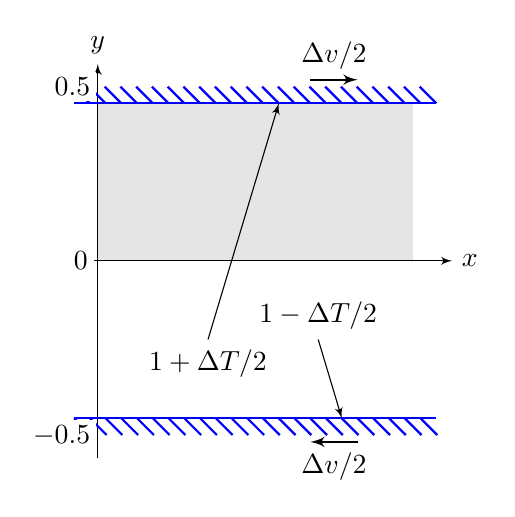
\begin{tikzpicture}[dashdot/.style={dash pattern=on .6pt off 1pt on 6pt off 1pt},
			interface/.style={postaction={draw, decorate, decoration=
				{border, angle=-45, amplitude=0.3cm, segment length=2mm}}},
			label/.style={fill=white, inner sep=2pt},
			>=latex', scale=1]
	\fill[gray!20] (0,2) -- (4,2) -- (4,4) -- (0,4) -- cycle;
	\draw[->] (-.05,2) -- (4.5,2) node[right] {\(x\)};
	\draw[->](0,-.5) -- (0,4.5) node[above] {\(y\)};
	\draw[blue, thick, interface](-.3,0) -- (4.3,0);
	\draw[blue, thick, interface](4.3,4) -- (-0.3,4);
	\draw[->] (1.4,1) node[below] {\(1+\Delta T/2\)} -- (2.3,4);
	\draw[->] (2.8,1) node[above] {\(1-\Delta T/2\)} -- (3.1,0);
    \draw[->, thick] (2.7,4.3) -- (3.3,4.3) node[midway,above] {\(\Delta v/2\)};
    \draw[<-, thick] (2.7,-.3) -- (3.3,-.3) node[midway,below] {\(\Delta v/2\)};
	\node at (-.02,-.02) [below left, label] {\(-0.5\)};
	\node at (-.02,4.02) [above left, label] {\(0.5\)};
	\node at (-.05,2) [left, label] {\(0\)};
\end{tikzpicture}

\end{document}
